
\documentclass[letterpaper,hide notes,xcolor={table,svgnames},pdftex,10pt]{beamer}
\def\showexamples{t}

\usecolortheme{crane}
\setbeamertemplate{navigation symbols}{}

\usetheme{MyPittsburgh}
\usepackage{hyperref}
\usepackage{graphicx,xspace}
\usepackage[normalem]{ulem}
\usepackage{multicol}
\usepackage{amsmath,amssymb,amsthm,graphicx,xspace}
\newcommand\SF[1]{$\bigstar$\footnote{SF: #1}}

\usepackage[sfdefault,lf]{carlito}
\usepackage[T1]{fontenc}
\usepackage[scaled]{beramono}
\usepackage{tikzpagenodes}
\newcommand{\Rplus}{\protect\hspace{-.1em}\protect\raisebox{.35ex}{\small{\small\textbf{+}}}}
\newcommand{\Cpp}{\mbox{C\Rplus\Rplus}\xspace}

\newcounter{tmpnumSlide}
\newcounter{tmpnumNote}

\newcommand\mnote[1]{%
	\addtocounter{tmpnumSlide}{1}
	\ifdefined\showcues {~\tiny\fbox{\arabic{tmpnumSlide}}}\fi
	\note{\setlength{\parskip}{1ex}\addtocounter{tmpnumNote}{1}\textbf{\Large \arabic{tmpnumNote}:} {#1\par}}}

\newcommand\mmnote[1]{\note{\setlength{\parskip}{1ex}#1\par}}


\newcommand\mquestion[2]{{~\color{red}\fbox{?}}\note{\setlength{\parskip}{1ex}\par{\Large \textbf{?}} #1} \note{\setlength{\parskip}{1ex}\par{\Large \textbf{A}} #2\par}\ifdefined \presentationonly \pause \fi}

\newcommand\blackboard[1]{%
	\ifdefined   \showblackboard
		{#1}
	\else {\begin{center} \fbox{\colorbox{blue!30}{%
						\begin{minipage}{.95\linewidth}%
							\hspace{\stretch{1}} Some space intentionally left blank; done at the blackboard.%
						\end{minipage}}}\end{center}}%
	\fi%
}

\usepackage{listings}
\lstset{%
	keywordstyle=\bfseries,
	aboveskip=15pt,
	belowskip=15pt,
	captionpos=b,
	identifierstyle=\ttfamily,
	frame=lines,
	numbers=left, basicstyle=\scriptsize, numberstyle=\tiny, stepnumber=0, numbersep=2pt}

\usepackage{siunitx}
\newcommand\sius[1]{\num[group-separator = {,}]{#1}\si{\micro\second}}
\newcommand\sims[1]{\num[group-separator = {,}]{#1}\si{\milli\second}}
\newcommand\sins[1]{\num[group-separator = {,}]{#1}\si{\nano\second}}
\sisetup{group-separator = {,}, group-digits = true}

%% -------------------- tikz --------------------
\usepackage{tikz}
\usetikzlibrary{positioning}
\usetikzlibrary{arrows,backgrounds,automata,decorations.shapes,decorations.pathmorphing,decorations.markings,decorations.text}

\tikzstyle{place}=[circle,draw=blue!50,fill=blue!20,thick, inner sep=0pt,minimum size=6mm]
\tikzstyle{transition}=[rectangle,draw=black!50,fill=black!20,thick, inner sep=0pt,minimum size=4mm]

\tikzstyle{block}=[rectangle,draw=black, thick, inner sep=5pt]
\tikzstyle{bullet}=[circle,draw=black, fill=black, thin, inner sep=2pt]

\tikzstyle{pre}=[<-,shorten <=1pt,>=stealth',semithick]
\tikzstyle{post}=[->,shorten >=1pt,>=stealth',semithick]
\tikzstyle{bi}=[<->,shorten >=1pt,shorten <=1pt, >=stealth',semithick]

\tikzstyle{mut}=[-,>=stealth',semithick]

\tikzstyle{treereset}=[dashed,->, shorten >=1pt,>=stealth',thin]

\usepackage{ifmtarg}
\usepackage{xifthen}
\makeatletter
% new counter to now which frame it is within the sequence
\newcounter{multiframecounter}
% initialize buffer for previously used frame title
\gdef\lastframetitle{\textit{undefined}}
% new environment for a multi-frame
\newenvironment{multiframe}[1][]{%
	\ifthenelse{\isempty{#1}}{%
		% if no frame title was set via optional parameter,
		% only increase sequence counter by 1
		\addtocounter{multiframecounter}{1}%
	}{%
		% new frame title has been provided, thus
		% reset sequence counter to 1 and buffer frame title for later use
		\setcounter{multiframecounter}{1}%
		\gdef\lastframetitle{#1}%
	}%
	% start conventional frame environment and
	% automatically set frame title followed by sequence counter
	\begin{frame}%
		\frametitle{\lastframetitle~{\normalfont(\arabic{multiframecounter})}}%
		}{%
	\end{frame}%
}
\makeatother

\makeatletter
\newdimen\tu@tmpa%
\newdimen\ydiffl%
\newdimen\xdiffl%
\newcommand\ydiff[2]{%
	\coordinate (tmpnamea) at (#1);%
	\coordinate (tmpnameb) at (#2);%
	\pgfextracty{\tu@tmpa}{\pgfpointanchor{tmpnamea}{center}}%
	\pgfextracty{\ydiffl}{\pgfpointanchor{tmpnameb}{center}}%
	\advance\ydiffl by -\tu@tmpa%
}
\newcommand\xdiff[2]{%
	\coordinate (tmpnamea) at (#1);%
	\coordinate (tmpnameb) at (#2);%
	\pgfextractx{\tu@tmpa}{\pgfpointanchor{tmpnamea}{center}}%
	\pgfextractx{\xdiffl}{\pgfpointanchor{tmpnameb}{center}}%
	\advance\xdiffl by -\tu@tmpa%
}
\makeatother
\newcommand{\copyrightbox}[3][r]{%
	\begin{tikzpicture}%
		\node[inner sep=0pt,minimum size=2em](ciimage){#2};
		\usefont{OT1}{phv}{n}{n}\fontsize{4}{4}\selectfont
		\ydiff{ciimage.south}{ciimage.north}
		\xdiff{ciimage.west}{ciimage.east}
		\ifthenelse{\equal{#1}{r}}{%
			\node[inner sep=0pt,right=1ex of ciimage.south east,anchor=north west,rotate=90]%
			{\raggedleft\color{black!50}\parbox{\the\ydiffl}{\raggedright{}#3}};%
		}{%
			\ifthenelse{\equal{#1}{l}}{%
				\node[inner sep=0pt,right=1ex of ciimage.south west,anchor=south west,rotate=90]%
				{\raggedleft\color{black!50}\parbox{\the\ydiffl}{\raggedright{}#3}};%
			}{%
				\node[inner sep=0pt,below=1ex of ciimage.south west,anchor=north west]%
				{\raggedleft\color{black!50}\parbox{\the\xdiffl}{\raggedright{}#3}};%
			}
		}
	\end{tikzpicture}
}


%% --------------------

%\usepackage[excludeor]{everyhook}
%\PushPreHook{par}{\setbox0=\lastbox\llap{MUH}}\box0}

%\vspace*{\stretch{1}

%\setbox0=\lastbox \llap{\textbullet\enskip}\box0}

\setlength{\parskip}{\fill}

\newcommand\noskips{\setlength{\parskip}{1ex}}
\newcommand\doskips{\setlength{\parskip}{\fill}}

\newcommand\xx{\par\vspace*{\stretch{1}}\par}
\newcommand\xxs{\par\vspace*{2ex}\par}
\newcommand\tuple[1]{\langle #1 \rangle}
\newcommand\code[1]{{\sf \footnotesize #1}}
\newcommand\ex[1]{\uline{Example:} \ifdefined \presentationonly \pause \fi
	\ifdefined\showexamples#1\xspace\else{\uline{\hspace*{2cm}}}\fi}

\newcommand\ceil[1]{\lceil #1 \rceil}


\AtBeginSection[]
{
	\begin{frame}
		\frametitle{Outline}
		\tableofcontents[currentsection]
	\end{frame}
}



\pgfdeclarelayer{edgelayer}
\pgfdeclarelayer{nodelayer}
\pgfsetlayers{edgelayer,nodelayer,main}

\tikzstyle{none}=[inner sep=0pt]
\tikzstyle{rn}=[circle,fill=Red,draw=Black,line width=0.8 pt]
\tikzstyle{gn}=[circle,fill=Lime,draw=Black,line width=0.8 pt]
\tikzstyle{yn}=[circle,fill=Yellow,draw=Black,line width=0.8 pt]
\tikzstyle{empty}=[circle,fill=White,draw=Black]
\tikzstyle{bw} = [rectangle, draw, fill=blue!20,
text width=4em, text centered, rounded corners, minimum height=2em]

\newcommand{\CcNote}[1]{% longname
	This work is licensed under the \textit{Creative Commons #1 3.0 License}.%
}
\newcommand{\CcImageBy}[1]{%
	\includegraphics[scale=#1]{creative_commons/cc_by_30.pdf}%
}
\newcommand{\CcImageSa}[1]{%
	\includegraphics[scale=#1]{creative_commons/cc_sa_30.pdf}%
}
\newcommand{\CcImageNc}[1]{%
	\includegraphics[scale=#1]{creative_commons/cc_nc_30.pdf}%
}
\newcommand{\CcGroupBySa}[2]{% zoom, gap
	\CcImageBy{#1}\hspace*{#2}\CcImageNc{#1}\hspace*{#2}\CcImageSa{#1}%
}
\newcommand{\CcLongnameByNcSa}{Attribution-NonCommercial-ShareAlike}

\newenvironment{changemargin}[1]{% 
	\begin{list}{}{% 
		\setlength{\topsep}{0pt}% 
		\setlength{\leftmargin}{#1}% 
		\setlength{\rightmargin}{1em}
		\setlength{\listparindent}{\parindent}% 
		\setlength{\itemindent}{\parindent}% 
		      \setlength{\parsep}{\parskip}% 
		      }% 
		\item[]}{\end{list}}




\title{Lecture 20 --- Disk Scheduling }

\author{Jeff Zarnett \\ \small \texttt{jzarnett@uwaterloo.ca}}
\institute{Department of Electrical and Computer Engineering \\
  University of Waterloo}
\date{\today}


\begin{document}

\begin{frame}
  \titlepage

 \end{frame}



\begin{frame}
\frametitle{Disk Scheduling}

The disk is a very slow device, as far as the CPU is concerned.

\begin{center}
	
\includegraphics[width=0.5\textwidth]{images/sloth.jpg}
\end{center}

We will examine the hardware behind magnetic disks and see why they are so slow and consider algorithms that could be used to speed up operations.

 \end{frame}

\begin{frame}
\frametitle{Magnetic Disks}

Unless you have a Solid State Drive, the mass and permanent storage of data in your system is on a magnetic hard disk. 

Due to the physical nature of how disk drives work, there is an associated delay with moving to a new location and reading the data there. 

Thus, we would like to devise efficient schedules for reading and writing.


\end{frame}

\begin{frame}
\frametitle{SSDs}

We will exclude SSDs from consideration here. 

\begin{center}
	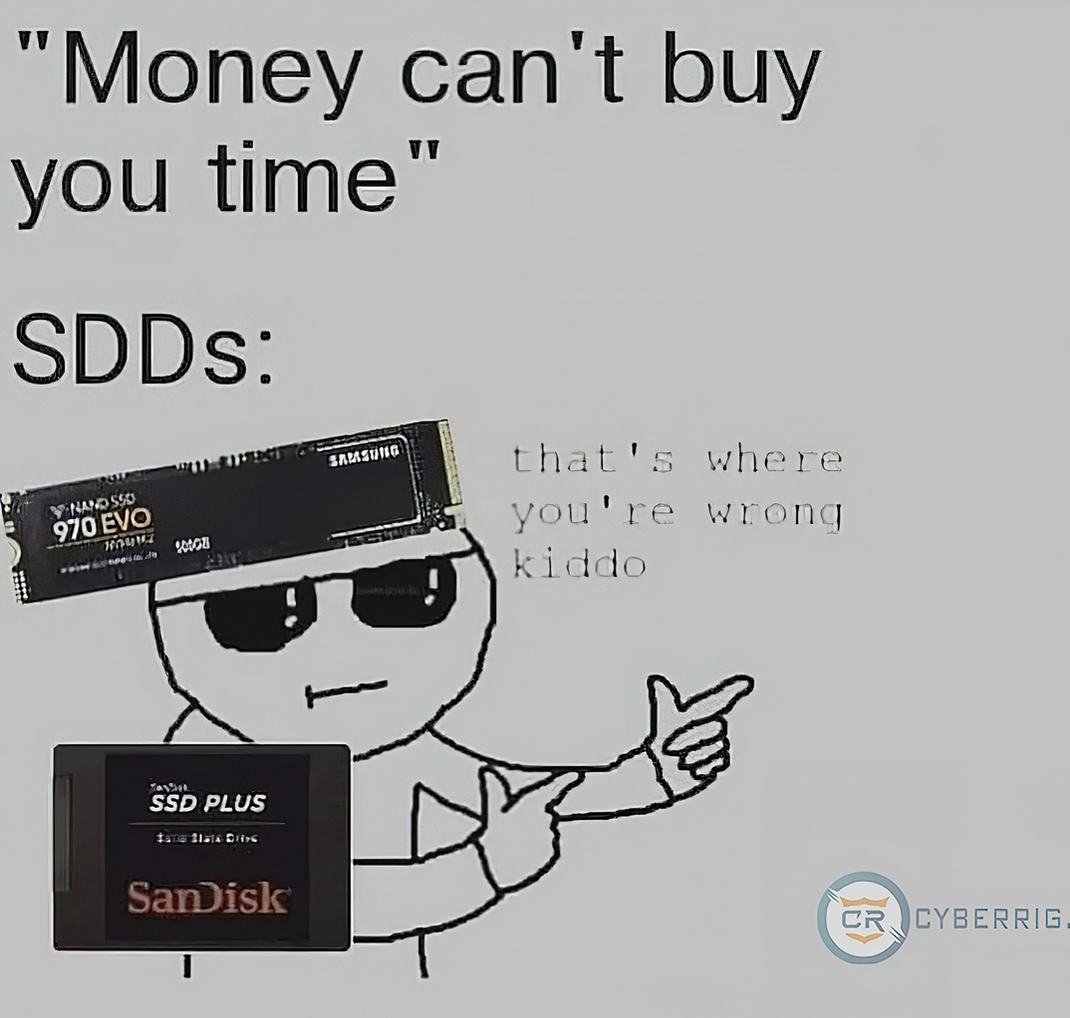
\includegraphics[width=0.5\textwidth]{images/ssd.png}
\end{center}

 \end{frame}

\begin{frame}
\frametitle{Magnetic Disks}

SSDs do not contain moving disk heads or spinning platters. 

An algorithm to schedule the optimal movement of the disk heads is irrelevant. 

Read access times from the SSD are consistent and uniform even if data is being requested from random locations. 

The SSD disk scheduling algorithm can be as simple as first-come, first-served.


\end{frame}

\begin{frame}
\frametitle{Disk Scheduling Motivation}

Why bother learning about this if magnetic drives are going away? 

The first is that while magnetic drives might be on the way out, they're not dead yet and many systems still use them, including large databases. 

The other is that disks are a convenient example, but not the only I/O device that needs to seek around to read and write data.

So what we examine here may be applicable to other sorts of devices too.

\end{frame}

\begin{frame}
\frametitle{Hard Drive Internals}

\begin{center}
	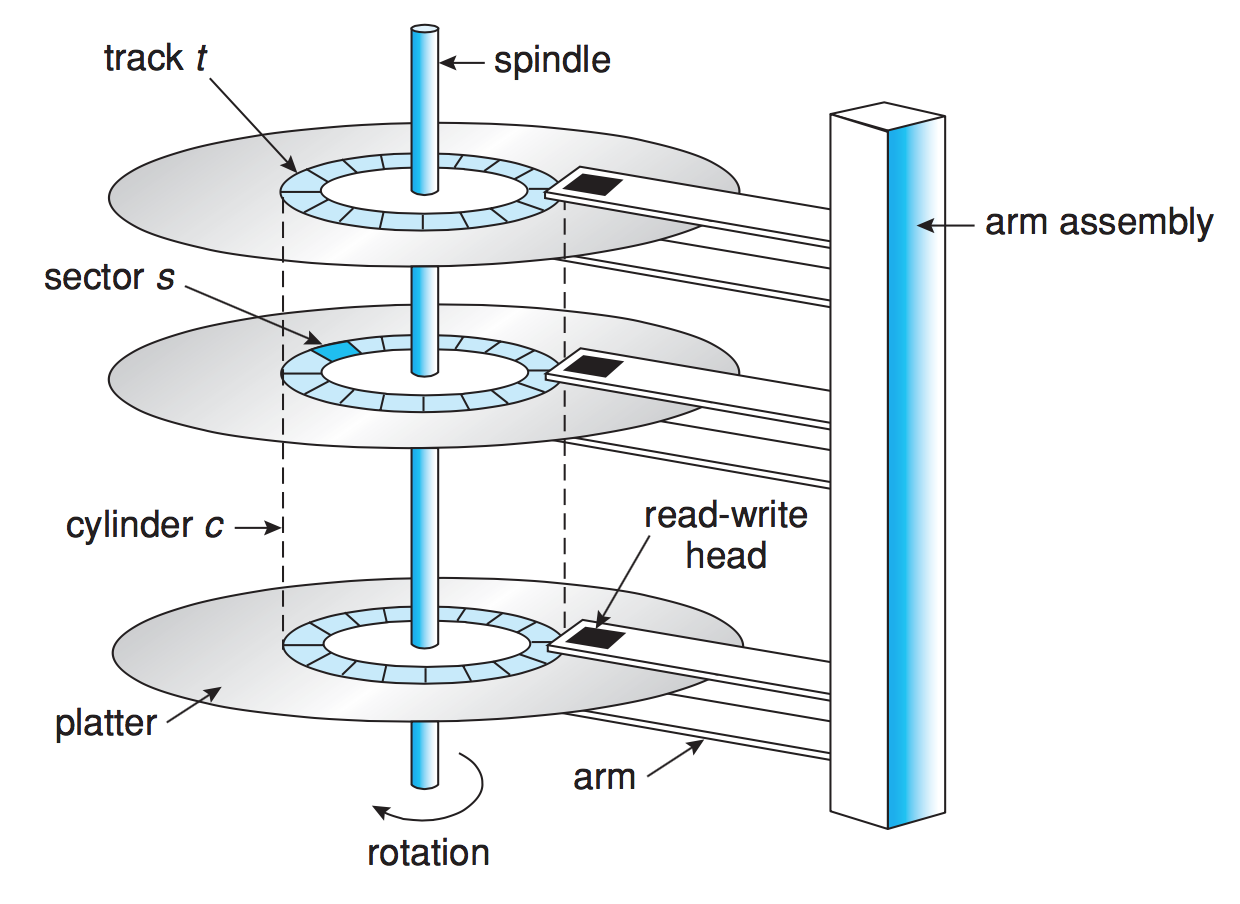
\includegraphics[width=0.75\textwidth]{images/disk-hardware.png}
\end{center}

\end{frame}

\begin{frame}
\frametitle{Don't Crash}

A read-write head is suspended a very small distance above the surface of each platter and reads or writes data directly beneath it. 

This is why they are carefully sealed: if a bit of dust lands on the platter, the read-write head can run into it (which is bad). 

It gets even worse if a disk head makes contact with the platter: this is called a head crash and it tends to permanently destroy data. 


\end{frame}

\begin{frame}
\frametitle{Platter Organization}

The platter surface is divided logically into different circular tracks, which are respectively divided up into sectors (blocks). 

A set of tracks stacked vertically is called a column. 

When the disk is in use, a motor spins the platters at high speed and another one manipulates the positions of the arm.


\end{frame}

\begin{frame}
\frametitle{Disk Performance}

The performance of the disk can be broken down into two values. 

The first is the \alert{transfer rate}; the speed at which data can be moved from the disk to the computer or vice-versa. 

The other is the \alert{random-access time}; how long it takes to get to a particular piece of data. 

The random access time itself is broken down into:\\
\quad The \alert{seek time} and the \alert{rotational latency}

Seek times and rational latencies tend to run in the millisecond range.


\end{frame}

\begin{frame}
\frametitle{Disk Transfer Time}

\begin{center}
	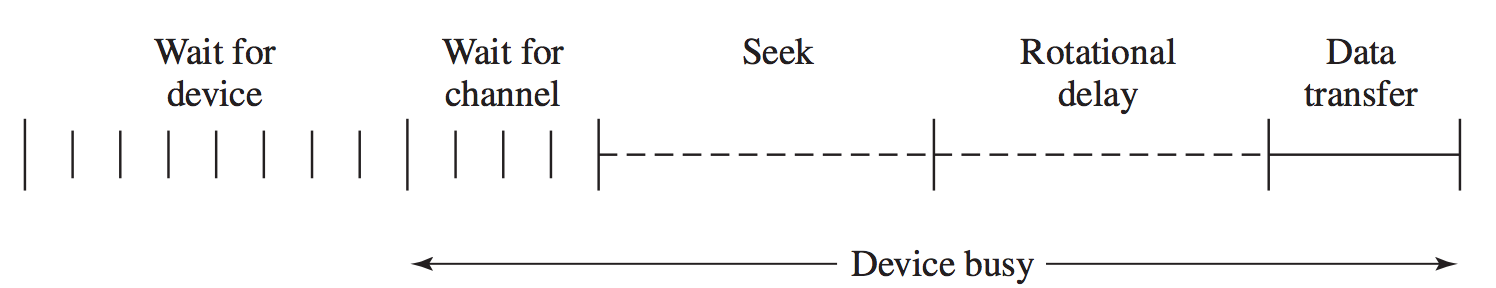
\includegraphics[width=0.9\textwidth]{images/disk-transfer-time.png}
\end{center}


\end{frame}

\begin{frame}
\frametitle{Disk Access Time}

The total average access time, $T_{a}$, for a disk operation:

\begin{center}
$T_{a} = T_{s} + \dfrac{1}{2r} + \dfrac{b}{rN}$
\end{center}

Where: $T_{s}$ is the average seek time\\
\quad $r$ is the rotation speed (revolutions per second)\\
\quad $b$ is the number of bytes to be transferred\\ 
\quad $N$ is the number of bytes on a track.


\end{frame}

\begin{frame}
\frametitle{Performance Variance}

A small example.

The disk has an average seek time of 4~ms, a rotation speed of 7~500 RPM, and 512-byte sectors with 500 sectors per track. 

We want to read a file that is 2~500 sectors (a total of 1.28~MB). 

\end{frame}

\begin{frame}
\frametitle{Performance Variance}

If the file is stored as compactly on disk as it can be, it is \alert{sequentially organized}: the file occupies all the sectors on 5 adjacent tracks. 

To read the first track, it will take 16~ms: 4~ms to seek, 4~ms rotational delay, and then 8~ms to read 500 sectors. 

Because the data is sequential, no additional seek time is necessary, so we just keep reading subsequent sectors which means only the rotational delay. 

Each additional track takes 12~ms (4~ms rotational delay + 8~ms to read it). Thus the total time is $16 + (4 \times 12)$ = 64~ms.

\end{frame}

\begin{frame}
\frametitle{Performance Variance}

What if instead the data was randomly distributed on the disk (not sequential)? 

The average seek and rotational delay times don't change. 

Reading one sector takes 0.016~ms. 

So each read of a sector will take a total of 8.016~ms ($4 + 4 + 0.016$).

There are 2~500 sectors so the total is $2~500 \times 8.016 =$ 20~040~ms. 

\end{frame}



\begin{frame}
\frametitle{THIS READ TIME IS...}

\begin{center}

\includegraphics[width=0.8\textwidth]{images/unacceptable}
\end{center}

\end{frame}

\begin{frame}
\frametitle{Performance Variance}

20~000~ms - twenty full seconds to read 1.28~MB of data? Yes. Seriously. 

This speed would be considered utterly unacceptable by the users. 

The order in which sectors are read from the disk makes a huge difference. 

Decisions about how to store data on disk is extremely important. 

Not only is placement important, but how we schedule the reads and writes.


\end{frame}

\begin{frame}
\frametitle{Disk Scheduling}

We should introduce a final metric, the \alert{bandwidth}. 

Bandwidth is the total number of bytes transferred, divided by the total time between the request for service and completion of the transfer. 

This is a measure of how much data is effectively transferred in a period of time. 

This is one of the measures we would like to improve, as well as the access time.

\end{frame}

\begin{frame}
\frametitle{Reading or Writing from Disk}

When a process needs to read from or write to the disk, the system call contains the following information:

\begin{enumerate}
	\item If the operation is a read or write.
	\item The disk address for the transfer.
	\item The memory address for the transfer.
	\item How much data to transfer (how many sectors).
\end{enumerate}

\end{frame}

\begin{frame}
\frametitle{Scheduling Algorithm: Random}

Nobody actually seriously advocates random scheduling, but it is a baseline against which to compare various scheduling algorithms. 

We could do disk accesses based on process priority, paying no attention to how (in)convenient it is from the perspective of the disk.

If there is only one request, there is not much of a decision to make.

\end{frame}

\begin{frame}
\frametitle{First-Come, First-Served}

Fair and simple, but does not necessarily provide the fastest service.

No attempt is made to group, organize, or rearrange the requests.

Example: requests for I/O to/from cylinders: \{98, 183, 37, 122, 14, 124, 65, 67\}; the disk head begins at 53.

\begin{center}
	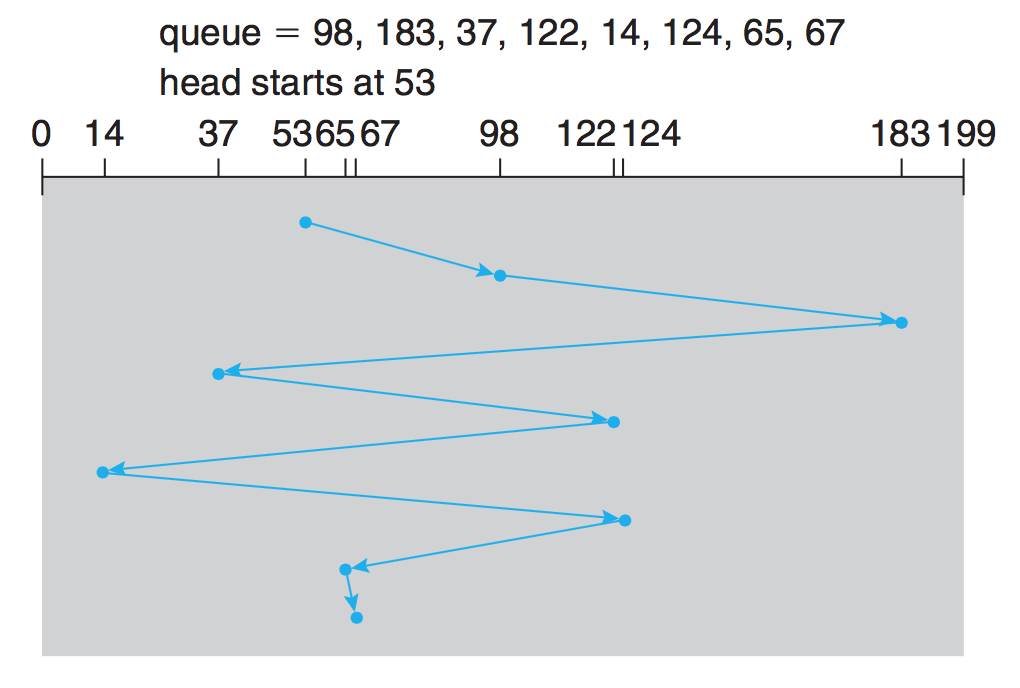
\includegraphics[width=0.5\textwidth]{images/disk-fcfs.png}
\end{center}

Total movement: 640 cylinders.

\end{frame}

\begin{frame}
\frametitle{Shortest Seek Time First}

Choose the request with the least seek time from the current head position.

\begin{center}
	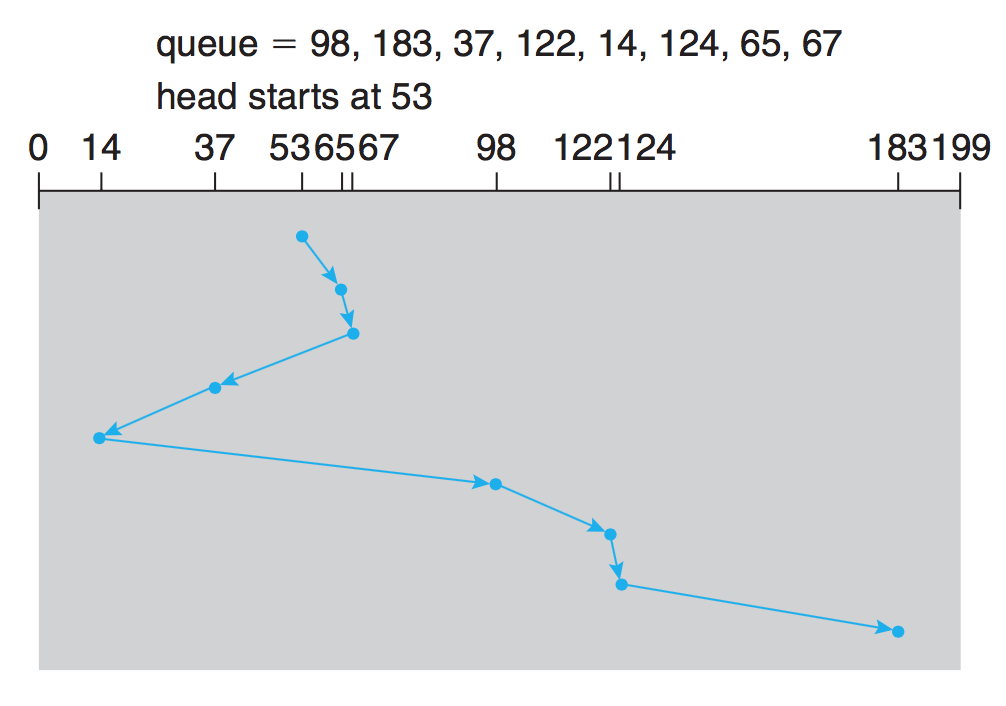
\includegraphics[width=0.5\textwidth]{images/disk-sstf.png}
\end{center}

Total movement: 236 cylinders.

\end{frame}

\begin{frame}
\frametitle{Shortest Seek Time First}

This routine is unfortunately subject to starvation. 

Suppose the disk head is at position 14. 

While is is there, a new request at 24 arrives, making the request at 98 wait. 

If enough low-numbered requests arrive to arrive during execution, a request at a high number may be put off, potentially indefinitely. 

The more requests occur, the more likely starvation is.

\end{frame}

\begin{frame}
\frametitle{Shortest Seek Time First}

Though the SSTF algorithm is an improvement, it is not optimal. 

In the example, we would reduce the total amount of movement to 208 cylinders if we did the move from 53 to 37, even though it is not the closest.

This algorithm provides for some spatial locality.

\end{frame}

\begin{frame}
\frametitle{SCAN Scheduling}

Move in one direction at a time until it reaches the ``end'' of the disk. 

After that, the direction is reversed. 

The SCAN algorithm is sometimes called the elevator algorithm.
\end{frame}

\begin{frame}
\frametitle{SCAN Scheduling}

If a request arrives just in front of the head (e.g, 129 arrives before 124 is serviced), it will be serviced virtually right away.

If it is just after where the head has been (e.g., 123 after 124 has been serviced) it will wait until the direction reverses again. 

\begin{center}
	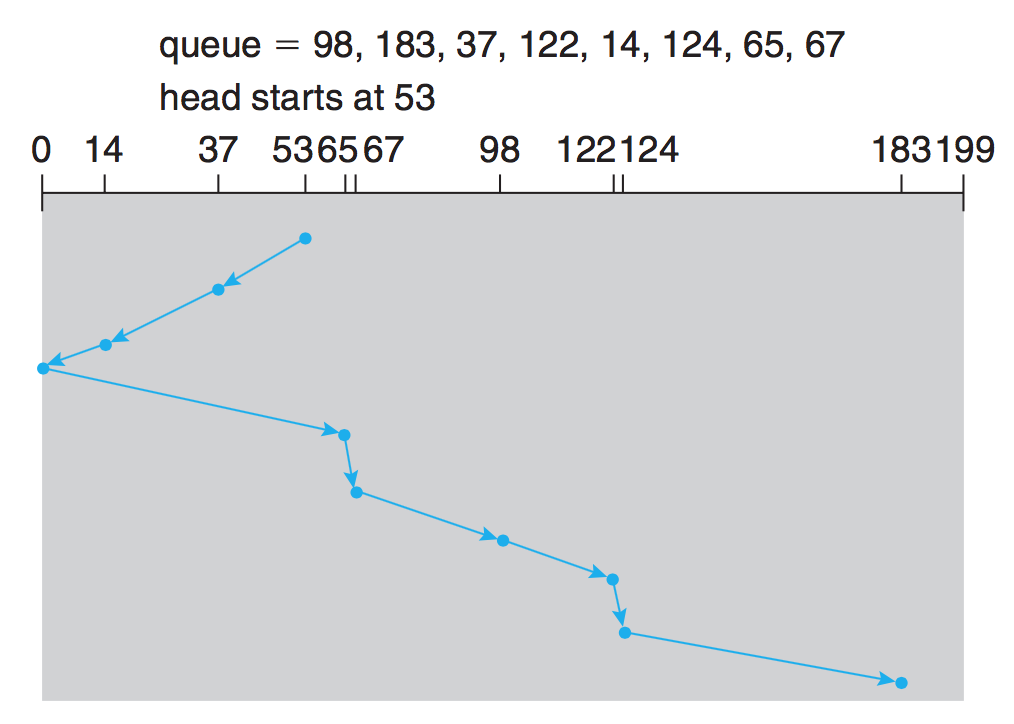
\includegraphics[width=0.5\textwidth]{images/disk-scan.png}
\end{center}


\end{frame}

\begin{frame}
\frametitle{SCAN Scheduling}

The SCAN policy does not take advantage of spatial locality as SSTF does. 

If the head has just moved from an area, it can be a long time before it returns.

Thus, if there are multiple accesses in the same area, they are likely to be at least partly spread out in time.

\end{frame}

\begin{frame}
\frametitle{C-SCAN Scheduling}

C-SCAN is designed to exploit the fact that when the disk has just reached one end, most requests are likely at the other end of the disk. 

So instead of reversing the direction and servicing requests on the way, jump back to the start of disk immediately and start at the beginning. 

It is called C-SCAN because C is for ``Circular'', as if the last cylinder just wraps around to the first.

\end{frame}

\begin{frame}
\frametitle{C-SCAN Scheduling}

\begin{center}
	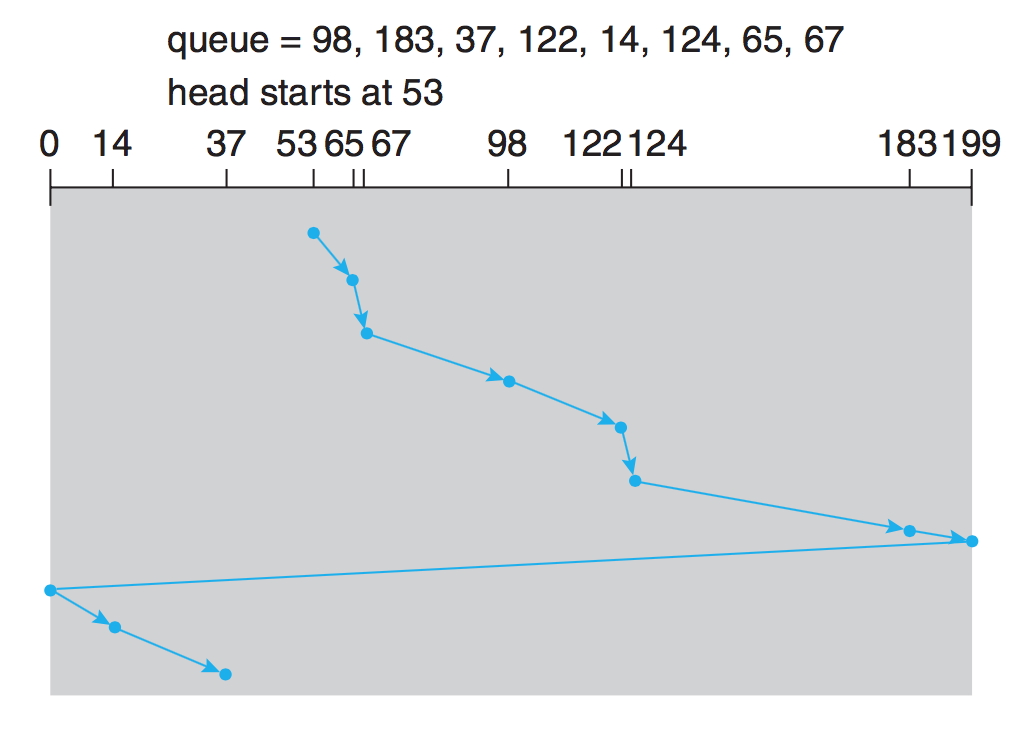
\includegraphics[width=0.5\textwidth]{images/disk-cscan.png}
\end{center}

Assume the amount of time it takes to scan from the start to end of disk is $t$. 

The expected service interval for sectors at the periphery is $2t$  with SCAN. 

C-SCAN reduces this to $t + s_{max}$ where $s_{max}$ is the maximum seek time.

\end{frame}

\begin{frame}
\frametitle{LOOK and C-LOOK}

The SCAN and C-SCAN algorithms as described can be optimized in a little way. 

Instead of going all the way to the end of disk every time, instead just go to the final request and only then reverse direction (or go back to the start). 

The names for this variant are LOOK and C-LOOK, respectively. 

\begin{center}
	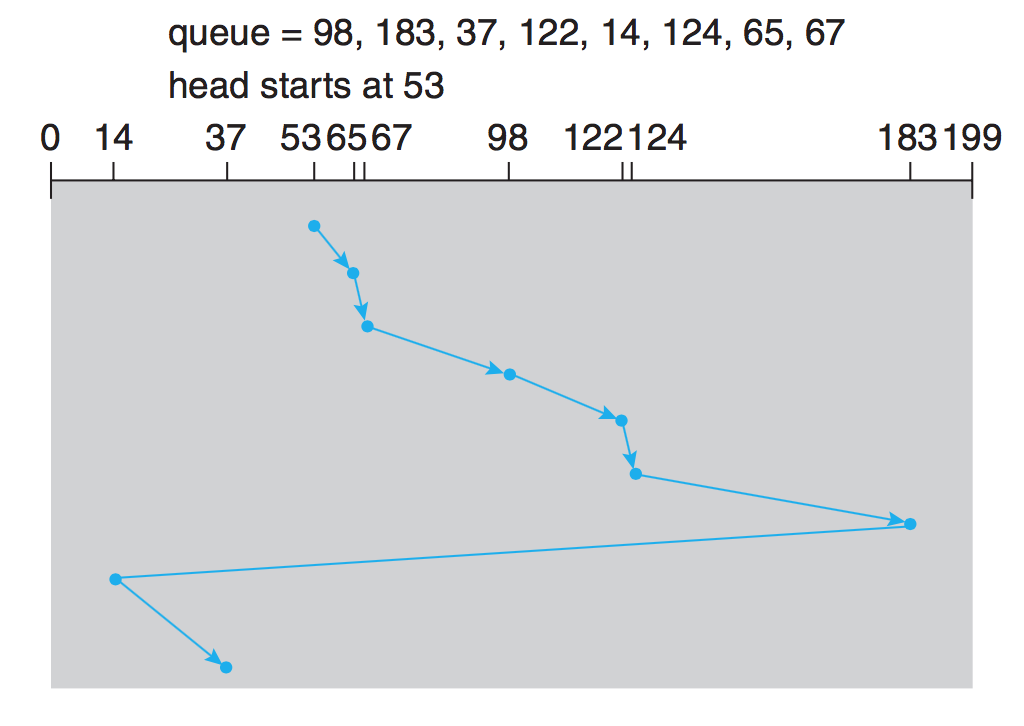
\includegraphics[width=0.5\textwidth]{images/disk-clook.png}
\end{center}



\end{frame}

\begin{frame}
\frametitle{Scheduling Algorithms}

We can probably agree that FCFS is not the best choice.

How do we decide between the other options?

The LOOK approach seems like it would prevent the starvation problem. 

Although we expect that with the SCAN or C-SCAN algorithm, all requests get serviced, it could happen that a process is effectively starved.

\end{frame}

\begin{frame}
\frametitle{Modification of SCAN}

A strategy to prevent this is a modification of the SCAN algorithm such that it has two queues for requests (think double buffering). 

While one queue is being emptied, the other is being filled. 

Thus, a request will not wait indefinitely; if the queue is of capacity $C$ then any particular read or write will wait, at most, $C$ accesses. 

The larger the value of $C$, the more the performance resembles SCAN; a smaller value of $C$ means behaviour is more like FCFS. 

The choice of $C$ is a tradeoff; sacrifice performance to increase fairness.


\end{frame}



\begin{frame}
\frametitle{Scheduling Algorithm Implementation}

The scheduling algorithms above consider only the seek times, and not the rotational latency, even though they can be about the same size. 

It is very difficult for the OS to schedule for improved rotational latency, because the disk is responsible for the physical placement of the logical blocks. 

The hard disk controller takes on some of the scheduling options. 

The OS can provide to the controller a grouping of requests, and then the controller will figure out how to schedule them.

\end{frame}

\begin{frame}
\frametitle{Scheduling Algorithm Choice}

If the speed of disk reads and writes were the only thing to be concerned about, the operating system would probably not worry about disk scheduling.

The OS may have certain priorities that should take precedence. 

\end{frame}

\begin{frame}
\frametitle{Scheduling Algorithm Choice}


Loading a page into main memory might need to take priority over an application writing a file to disk. 

Higher priority processes, especially in real-time systems, should not be waiting (for too long at least) for lower priority processes' disk writes. 

So, under some circumstances, the operating system needs to manage the reads and writes and not just leave it up to the disk controller.

\end{frame}

\end{document}

